\documentclass[11pt]{article}
\usepackage[a4paper,margin=2.4cm]{geometry}
\usepackage{pgfplots}
\pgfplotsset{compat=1.18}
\usepackage{pgf-pie}
\usepackage{booktabs}
\usepackage{xcolor}
\usepackage{caption}
\usepackage{enumitem}
\usepackage[hidelinks]{hyperref}

\captionsetup{font=small,labelfont=bf}
\pgfplotsset{
  barstyle/.style={ybar, bar width=8pt, ymin=0, width=\linewidth, height=5.2cm,
    enlarge x limits=0.06, axis x line*=bottom, axis y line*=left,
    ymajorgrids, grid style={gray!20},
    x tick label style={rotate=38,anchor=east,font=\scriptsize},
    y tick label style={font=\scriptsize}},
}

% tool-name shorthands (keep underscores out of prose)
\newcommand{\tl}[1]{\texttt{#1}}
\newcommand{\rstart}{\tl{rocq\_start}}
\newcommand{\rcheck}{\tl{rocq\_check}}
\newcommand{\rquery}{\tl{rocq\_query}}
\newcommand{\rstep}{\tl{rocq\_step\_multi}}
\newcommand{\rcompile}{\tl{rocq\_compile}}
\newcommand{\rcompilef}{\tl{rocq\_compile\_file}}
\newcommand{\rverify}{\tl{rocq\_verify}}
\newcommand{\rassum}{\tl{rocq\_assumptions}}
\newcommand{\rnot}{\tl{rocq\_notations}}
\newcommand{\rtoc}{\tl{rocq\_toc}}

% AUTO-GENERATED by parse.py — do not edit by hand.
\newcommand{\Ntotal}{1997}
\newcommand{\Ntranscripts}{580}
\newcommand{\Nmain}{422}
\newcommand{\Nsub}{158}
\newcommand{\Nmaincalls}{38}
\newcommand{\Nsubcalls}{1959}
\newcommand{\Subpct}{98.1}
\newcommand{\Nmatched}{1997}
\newcommand{\Nunmatched}{0}
\newcommand{\Nsucc}{1208}
\newcommand{\Nfail}{778}
\newcommand{\Nunknown}{11}
\newcommand{\Succpct}{60.8}
\newcommand{\Forcerestart}{80}
\newcommand{\Latdropped}{0}
\newcommand{\Dupcollapsed}{0}
\newcommand{\Ftooldefect}{303}
\newcommand{\Fusage}{166}
\newcommand{\Flegit}{49}
\newcommand{\Fambig}{260}
\newcommand{\Ffail}{778}
\newcommand{\Ftooldefectpct}{38.9}
\newcommand{\Flegitpct}{6.3}
\newcommand{\Nnode}{245}
\newcommand{\Ntimeout}{53}
\newcommand{\Qbroken}{150}
\newcommand{\Qtotal}{150}
\newcommand{\Asmbroken}{21}
\newcommand{\Asmtotal}{21}
\newcommand{\Checkn}{1300}
\newcommand{\Checksucc}{66}
\newcommand{\Checkmed}{0.024}
\newcommand{\Startptimeout}{30.1}
\newcommand{\SMcallrate}{89}
\newcommand{\SMtacrate}{41}
\newcommand{\SMtacn}{389}
\newcommand{\ChartToolVolPie}{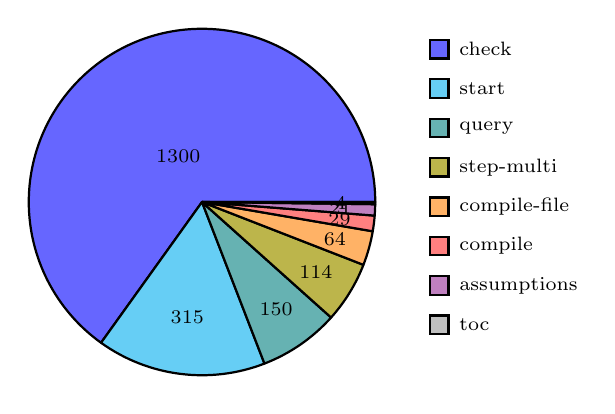
\begin{tikzpicture}\pie[radius=2.2,text=legend,sum=auto,font=\scriptsize,color={blue!60,cyan!60,teal!60,olive!60,orange!60,red!50,violet!50,gray!50}]{1300/check, 315/start, 150/query, 114/step-multi, 64/compile-file, 29/compile, 21/assumptions, 4/toc}\end{tikzpicture}}
\newcommand{\ChartFailPie}{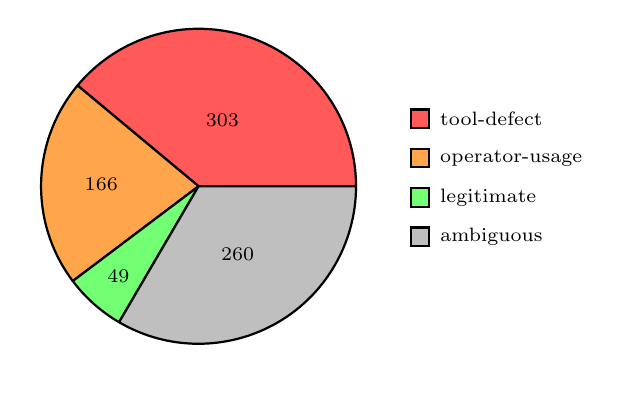
\begin{tikzpicture}\pie[radius=2.0,text=legend,sum=auto,font=\scriptsize,color={red!65,orange!70,green!55,black!25}]{303/tool-defect, 166/operator-usage, 49/legitimate, 260/ambiguous}\end{tikzpicture}}
\newcommand{\ErrBarCoords}{(0,245) (1,163) (2,122) (3,97) (4,53) (5,49) (6,43) (7,5) (8,1)}
\newcommand{\ErrBarLabels}{No node at point,Other,Syntax/parse,Reference/theorem not found,Timeout,Proof-state (apply/unify/unfinished),Focus discipline,Restart-through-Load,Notation ambiguity}
\newcommand{\ErrBarTick}{0,1,2,3,4,5,6,7,8}
\newcommand{\DaySuccCoords}{(0,490) (1,474) (2,135) (3,19) (4,15) (5,13) (6,11) (7,11) (8,38) (9,2)}
\newcommand{\DayFailCoords}{(0,352) (1,275) (2,92) (3,14) (4,0) (5,13) (6,5) (7,0) (8,24) (9,3)}
\newcommand{\DayLabels}{05-13,05-14,05-15,05-19,05-22,05-23,05-24,05-25,05-28,06-01}
\newcommand{\DayTick}{0,1,2,3,4,5,6,7,8,9}
\newcommand{\LatMedCoords}{(0,0.02) (1,0.28) (2,0.14) (3,0.05) (4,5.54) (5,5.24) (6,0.14) (7,0.16)}
\newcommand{\LatPCoords}{(0,0.07) (1,30.10) (2,5.04) (3,0.27) (4,6.94) (5,6.11) (6,6.68) (7,0.48)}
\newcommand{\LatLabels}{check,start,query,step-multi,compile-file,compile,assumptions,toc}
\newcommand{\LatTick}{0,1,2,3,4,5,6,7}
\newcommand{\SessBarCoords}{(1500,0) (324,1) (130,2) (33,3) (5,4) (5,5)}
\newcommand{\SessLabels}{DSDP secrecy + entropy,DSDP secrecy (PISMC),DSDP IND-CPA shell/trace,DSDP Charlie game-equiv,main-thread / misc,SMC interp. soundness}
\newcommand{\SessTick}{0,1,2,3,4,5}
\newcommand{\SessLegend}{\item \textbf{DSDP secrecy + entropy} (\texttt{sprightly-finding-robin}, 1500 calls, 60\% ok): DSDP Alice-secrecy: V2-aware SSProve chain, concrete corollaries, and entropy-form bound (dsdp\_alice\_secrecy\_indcpa, secrecy\_random\_guess). \item \textbf{DSDP secrecy (PISMC)} (\texttt{read-plan-claude-plans-sprightly-finding-vast-coral}, 324 calls, 60\% ok): Continuation of the secrecy plan: the PISMC variant of the chain (game\_real\_eq\_pismc, dsdp\_alice\_secrecy\_pismc, entropy\_ge\_bound\_pismc). \item \textbf{DSDP IND-CPA shell/trace} (\texttt{transient-juggling-flurry}, 130 calls, 68\% ok): DSDP IND-CPA shell-link and trace-bridge lemmas (valid\_boolean\_shell\_link, log\_id, alice\_trace\_eq\_concrete). \item \textbf{DSDP Charlie game-equiv} (\texttt{so-according-to-what-fluttering-goose}, 33 calls, 58\% ok): DSDP Charlie game-equivalence (game\_real\_equiv\_charlie\_real); session also covered merged-flow workflow planning. \item \textbf{main-thread / misc} (\texttt{(no slug)}, 5 calls, 20\% ok): Main-thread direct calls with no recorded session slug. \item \textbf{SMC interp. soundness} (\texttt{focus-on-the-rstep-squishy-alpaca}, 5 calls, 40\% ok): SMC interpreter rstep soundness port between branches (smc/smc\_interpreter\_sound.v).}
\newcommand{\SessAnno}{\node[anchor=west,font=\tiny] at (axis cs:1500,0) {60\%}; \node[anchor=west,font=\tiny] at (axis cs:324,1) {60\%}; \node[anchor=west,font=\tiny] at (axis cs:130,2) {68\%}; \node[anchor=west,font=\tiny] at (axis cs:33,3) {58\%}; \node[anchor=west,font=\tiny] at (axis cs:5,4) {20\%}; \node[anchor=west,font=\tiny] at (axis cs:5,5) {40\%};}
\newcommand{\ChartAttrPie}{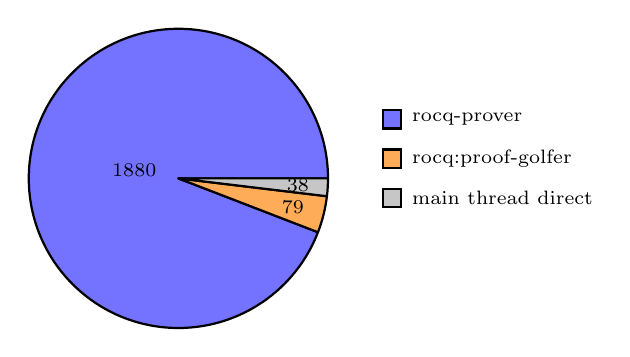
\begin{tikzpicture}\pie[radius=1.9,text=legend,sum=auto,font=\scriptsize,color={blue!55,orange!65,gray!45}]{1880/rocq-prover, 79/rocq:proof-golfer, 38/main thread direct}\end{tikzpicture}}
\newcommand{\AttrTableRows}{rocq-prover & 1880 & 59.9\% \\ rocq:proof-golfer & 79 & 77.2\% \\ (main thread, direct) & 38 & 52.6\% \\}
\newcommand{\SuccRateCoords}{(0,66.4) (1,56.4) (2,0.0) (3,97.1) (4,54.7) (5,93.1) (6,0.0) (7,100.0)}
\newcommand{\SuccRateLabels}{check,start,query,step-multi,compile-file,compile,assumptions,toc}
\newcommand{\SuccRateTick}{0,1,2,3,4,5,6,7}
\newcommand{\ToolTableRows}{check & 1300 & 863 & 436 & 1 & 0 & 66.4\% & 0.02 \\
start & 315 & 177 & 137 & 1 & 0 & 56.4\% & 0.28 \\
query & 150 & 0 & 150 & 0 & 0 & 0.0\% & 0.14 \\
step-multi & 114 & 102 & 3 & 9 & 0 & 97.1\% & 0.05 \\
compile-file & 64 & 35 & 29 & 0 & 0 & 54.7\% & 5.54 \\
compile & 29 & 27 & 2 & 0 & 0 & 93.1\% & 5.24 \\
assumptions & 21 & 0 & 21 & 0 & 0 & 0.0\% & 0.14 \\
toc & 4 & 4 & 0 & 0 & 0 & 100.0\% & 0.16 \\
verify & 0 & 0 & 0 & 0 & 0 & 0.0\% & 0.00 \\
notations & 0 & 0 & 0 & 0 & 0 & 0.0\% & 0.00 \\}
\newcommand{\RecoveryRows}{retry from\_state & 416 \\ different input, same tool & 193 \\ switched tool & 106 \\ force\_restart & 49 \\ abandoned (no further rocq call) & 14 \\}
\newcommand{\Stuckcount}{81}
\newcommand{\Stuckmax}{10}


\title{\textbf{A rocq-mcp Usage Retrospective}\\[2pt]
\large Empirical analysis of \Ntotal{} tool calls in the \texttt{infotheo-itp} project}
\author{Generated from Claude Code session transcripts}
\date{Corpus window 2026-05-08 to 2026-06-01 \quad|\quad Compiled 2026-06-03}

\begin{document}
\maketitle

\begin{abstract}
\noindent This is a one-time, evidence-based retrospective on how the
\textsf{rocq-mcp} MCP server was used while formalising the \texttt{infotheo-itp}
project. We parsed \Ntranscripts{} session transcripts (\Nmain{} main-thread,
\Nsub{} subagent) and extracted every \textsf{rocq-mcp} tool call joined to its
result: \Ntotal{} calls in all. The report is deliberately balanced. It separates
the server's own \emph{defects} from the operator's \emph{usage patterns}, and it
carves out \emph{legitimate proof-state failures} (a tactic that simply did not
close a goal) as nobody's fault. The headline: one workhorse tool (\rcheck) carried
the project at sub-second latency, while a positioning defect silently disabled
three read-only tools for the entire window.
\end{abstract}

\section*{0\quad Method note}
\addcontentsline{toc}{section}{Method note}
A ``call'' is a transcript \texttt{tool\_use} block whose name begins with
\texttt{mcp\_\_rocq-mcp\_\_}, joined to its \texttt{tool\_result} by
\texttt{tool\_use\_id}; we never count tool names mentioned in prose. Counting only
the main-thread transcripts would have found just \Nmaincalls{} calls; recursing
into the \texttt{subagents/} directories finds \Ntotal{} (a \(\sim\)50$\times$
correction), because \Subpct\,\% of all calls were delegated to subagents. Every
call matched a result (\Nunmatched{} unmatched, \Dupcollapsed{} duplicate ids
collapsed). A call counts as a success when its result carries
\texttt{success:true}; query-style results without a \texttt{success} field are
inferred from the absence of an error (\Nunknown{} remained unknown). Per-call
\emph{latency} is the wall-clock gap between the call's timestamp and its result's
timestamp; it includes harness overhead, so read it as approximate
(\Latdropped{} out-of-range outliers dropped). The classification of a failure as
\emph{tool-defect}, \emph{operator-usage}, \emph{legitimate-proof-state}, or
\emph{ambiguous} is a best-effort regex over the error text, audited by sampling;
the \emph{ambiguous} bucket is left honestly large rather than force-fitted.

\section*{1\quad Executive summary}
\addcontentsline{toc}{section}{Executive summary}
\begin{itemize}[leftmargin=1.4em,itemsep=2pt]
\item \textbf{Volume \& delegation.} \Ntotal{} calls; \Subpct\,\% ran inside
subagents, almost all (\(94\%\)) under a single \textsf{rocq-prover} agent. The
operator drove the prover by delegation, not by hand.
\item \textbf{One tool does the work.} \rcheck{} alone is \Checkn{} calls
(\(65\%\) of everything) at a median of \Checkmed\,s. It is the iteration engine;
the rest is setup and search.
\item \textbf{A defect disabled whole tools.} The ``No node at point'' positioning
bug (coq-lsp \(\ge 0.2.4\), patched only on 2026-06-02, \emph{after} this window)
accounts for \Nnode{} failures and rendered \rquery{} (\Qbroken/\Qtotal) and
\rassum{} (\Asmbroken/\Asmtotal) \emph{100\,\% non-functional}.
\item \textbf{The workhorse was reliable.} \rcheck{} took \(\Checksucc\,\%\) of its
calls to success and had essentially zero ``No node'' failures: its failures are
the proof work itself, not the tool.
\item \textbf{Big files time out.} \Ntimeout{} timeouts, mostly \rstart{} on large
files (its p90 latency is \Startptimeout\,s, right at the 30\,s ceiling).
\item \textbf{Two safety tools went unused.} \rverify{} and \rnot{} were never
called (0 each), so the axiom/statement-mismatch safety net was never engaged.
\item \textbf{Recovery was healthy.} After a failure the next move was most often a
principled backtrack (\texttt{from\_state}); only \(14\) failures were truly
abandoned. But \Stuckcount{} runs of \(\ge 3\) consecutive failures occurred, the
worst \Stuckmax{} long.
\end{itemize}

\section{Usage profile}
Figure~\ref{fig:toolpie} shows where the calls went. \rcheck{} dominates, with
\rstart{} and \rquery{} next; the heavyweight batch tools (\rcompile,
\rcompilef) are used sparingly, as intended. Figure~\ref{fig:attrpie} shows who
made the calls: delegation to \textsf{rocq-prover} is near-total.

\begin{figure}[h]\centering
\begin{minipage}{0.52\linewidth}\centering
\ChartToolVolPie
\captionof{figure}{Call volume by tool. \rcheck{} is \(65\%\) of all
\textsf{rocq-mcp} traffic.}\label{fig:toolpie}
\end{minipage}\hfill
\begin{minipage}{0.44\linewidth}\centering
\ChartAttrPie
\captionof{figure}{Calls by agent type. Almost everything is delegated to
\textsf{rocq-prover}.}\label{fig:attrpie}
\end{minipage}
\end{figure}

\noindent\textbf{Unused tools.} \rverify{}, \rnot{} (0 calls) and \rtoc{} (4
calls) are effectively dormant. \rverify{} in particular is the server's guard
against custom axioms and statement mismatch; leaving it unused means that check
fell entirely to the separate audit stage.

\section{Reliability}
Figure~\ref{fig:succ} gives the per-tool success rate. The two \(0\%\) bars
(\rquery, \rassum) are not noise: every one of their calls failed, all to the same
positioning defect (\S\ref{sec:err}). The reliable tools are \rtoc{} (\(100\%\)),
\rstep{} (\(97\%\)) and \rcompile{} (\(93\%\)); the workhorse \rcheck{} sits at
\(\Checksucc\%\), which is healthy given that its ``failures'' are mostly
in-progress proof states.

\begin{figure}[h]\centering
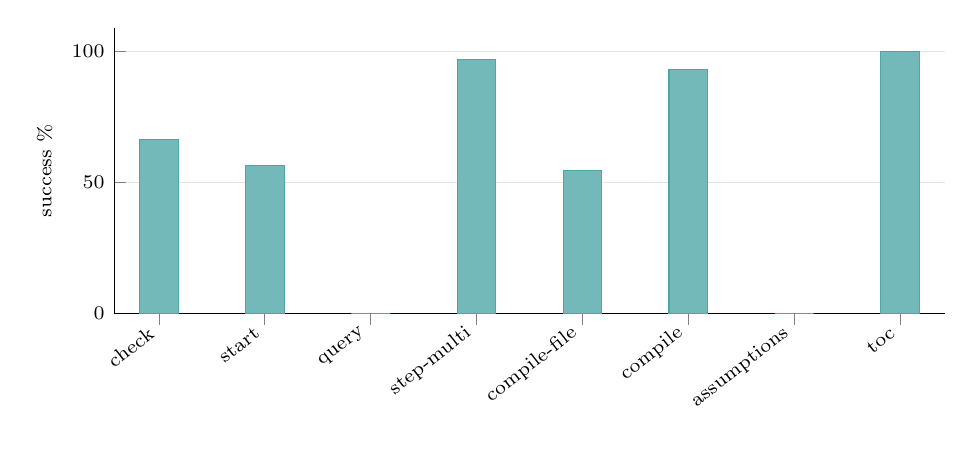
\begin{tikzpicture}
\begin{axis}[barstyle, bar width=14pt, ymax=109, ylabel={\scriptsize success \%},
  xtick=data, xticklabels/.expanded={\SuccRateLabels},
  nodes near coords, every node near coord/.append style={font=\tiny,rotate=90,anchor=west},
  point meta=explicit symbolic]
\addplot+[fill=teal!55,draw=teal!70] coordinates {\SuccRateCoords};
\end{axis}
\end{tikzpicture}
\captionof{figure}{Per-tool success rate (matched calls). \rquery{} and \rassum{}
are at \(0\%\) for the whole window.}\label{fig:succ}
\end{figure}

\noindent\textbf{Batch exploration.} \rstep{} shows the value of non-destructive
probing: \SMcallrate\,\% of \emph{calls} succeed even though only \SMtacrate\,\% of
the \SMtacn{} individual tactics tried actually applied. The tool is meant to spray
candidate tactics and keep the one that sticks, and that is exactly the observed
pattern.

\section{Error taxonomy}\label{sec:err}
Figure~\ref{fig:errbar} ranks the \Nfail{} failures by category. ``No node at
point'' is the single largest, ahead of generic compile/\emph{Other} errors,
syntax errors, and reference-not-found.

\begin{figure}[h]\centering
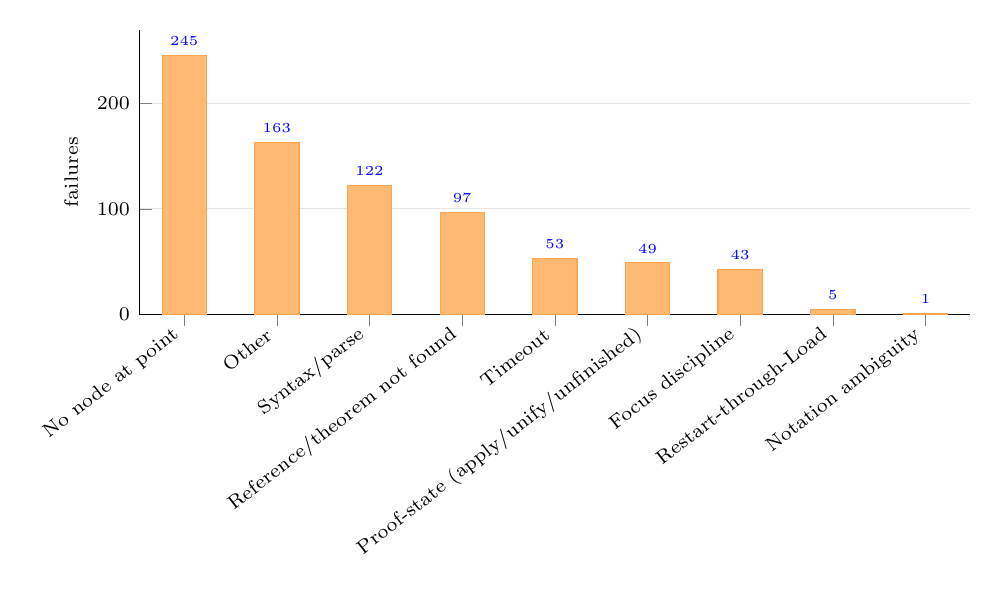
\begin{tikzpicture}
\begin{axis}[barstyle, bar width=16pt, ylabel={\scriptsize failures},
  xtick=data, xticklabels/.expanded={\ErrBarLabels},
  nodes near coords, every node near coord/.append style={font=\tiny}]
\addplot+[fill=orange!55,draw=orange!70] coordinates {\ErrBarCoords};
\end{axis}
\end{tikzpicture}
\captionof{figure}{Failures by error category across all tools.}\label{fig:errbar}
\end{figure}

\noindent Read per tool, the categories tell a sharp story. Of \rcheck's
failures, \emph{none} are ``No node at point'' (it works from an established proof
state and is immune); they are syntax, reference, focus, and genuine
apply/unify failures. By contrast \rquery{} (\(145\) of \(150\)) and \rassum{}
(\(19\) of \(21\)) are almost purely ``No node at point'', and \(81\) of \rstart's
\(137\) failures are the same defect. Hot-spot files were the SSProve wiring file
\texttt{smc/pismc\_to\_ssprove.v} and \texttt{dsdp\_security\_indcpa.v}.

\section{Defects versus usage}
Figure~\ref{fig:failpie} splits the failures by attribution.

\begin{figure}[h]\centering
\ChartFailPie
\captionof{figure}{Failure attribution. \emph{Legitimate} = a tactic that simply
did not close a goal (no one's fault). The \emph{ambiguous} slice is mixed and
deliberately not force-classified.}\label{fig:failpie}
\end{figure}

\noindent Confidently attributable tool defects total \Ftooldefect{}
(\Ftooldefectpct\,\% of failures): \Nnode{} positioning errors, \Ntimeout{}
timeouts, and a handful of ``Restart through Load'' edge cases. Confidently
legitimate proof-state failures total only \Flegit{} (\Flegitpct\,\%), but this is
a \emph{lower bound}: much of the \Fambig-strong \emph{ambiguous} bucket
(reference-not-found, proof-search-failed, mid-development compile errors) is also
ordinary proving. The honest reading is therefore: the defect share is real and
concentrated in the setup/query tools, the workhorse \rcheck{} is almost
defect-free, and a large remainder is the messy-but-normal cost of writing proofs.
One caveat trims the defect figure: a fraction of \rstart's ``No node'' results can
mean ``you started on a line with an earlier error'' rather than the coq-lsp bug,
so \Ftooldefect{} is an upper bound on genuine tool defects.

\section{Timing and activity}
Figure~\ref{fig:lat} (log scale) is the clearest validation of the intended
verification ladder: \rcheck{} returns in \(\sim\Checkmed\,\)s, an order of
magnitude faster than the batch compilers (\(\sim 5.5\,\)s), so cheap iteration
genuinely was cheap. The p90 markers expose the timeout cliff: \rstart{} reaches
the 30\,s ceiling. Figure~\ref{fig:timeline} shows the work was bursty, with the
overwhelming majority of all calls on 2026-05-13/14.

\begin{figure}[h]\centering
\begin{minipage}{0.5\linewidth}\centering
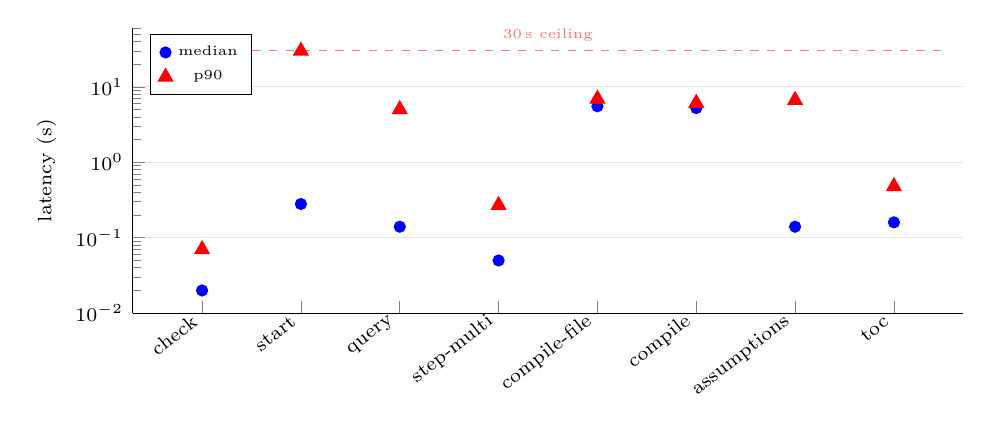
\begin{tikzpicture}
\begin{axis}[width=\linewidth,height=5.2cm,ymode=log,ymin=0.01,ymax=60,
  ylabel={\scriptsize latency (s)}, axis x line*=bottom, axis y line*=left,
  ymajorgrids, grid style={gray!20},
  xtick=data, xticklabels/.expanded={\LatLabels},
  x tick label style={rotate=38,anchor=east,font=\scriptsize},
  y tick label style={font=\scriptsize}, legend style={font=\tiny,at={(0.02,0.98)},anchor=north west}]
\addplot[only marks,mark=*,mark size=2pt,blue] coordinates {\LatMedCoords};
\addplot[only marks,mark=triangle*,mark size=3pt,red] coordinates {\LatPCoords};
\draw[dashed,red!55] (axis cs:-0.5,30) -- (axis cs:7.5,30)
  node[pos=0.5,above,font=\tiny]{30\,s ceiling};
\legend{median,p90}
\end{axis}
\end{tikzpicture}
\captionof{figure}{Per-call latency by tool (log).}\label{fig:lat}
\end{minipage}\hfill
\begin{minipage}{0.48\linewidth}\centering
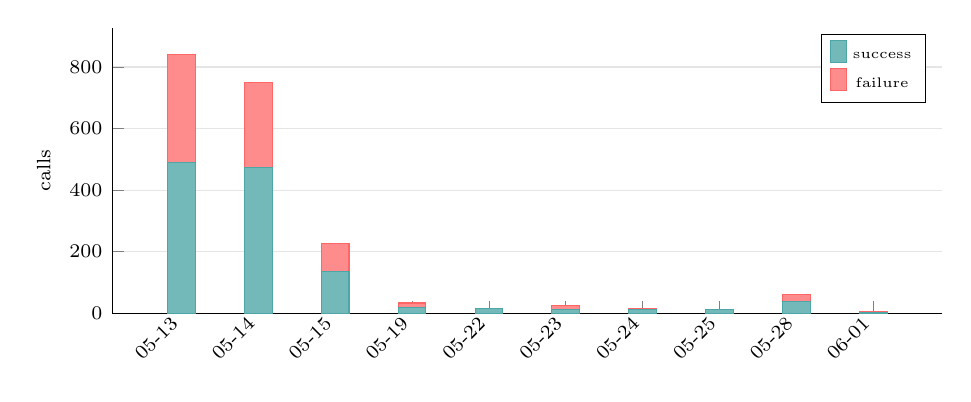
\begin{tikzpicture}
\begin{axis}[ybar stacked, bar width=10pt, width=\linewidth,height=5.2cm,ymin=0,
  axis x line*=bottom, axis y line*=left, ymajorgrids, grid style={gray!20},
  ylabel={\scriptsize calls}, xtick=data, xticklabels/.expanded={\DayLabels},
  x tick label style={rotate=45,anchor=east,font=\scriptsize},
  y tick label style={font=\scriptsize}, legend style={font=\tiny,at={(0.98,0.98)},anchor=north east}]
\addplot+[fill=teal!55,draw=teal!70] coordinates {\DaySuccCoords};
\addplot+[fill=red!45,draw=red!60] coordinates {\DayFailCoords};
\legend{success,failure}
\end{axis}
\end{tikzpicture}
\captionof{figure}{Daily activity (success vs failure).}\label{fig:timeline}
\end{minipage}
\end{figure}

\section{Recovery, friction, and sessions}
Table~\ref{tab:rec} shows what happened on the call immediately after a failure.
Principled backtracking with \texttt{from\_state} is the dominant response, which
is the behaviour the API documentation recommends; only \(14\) failures ended a
tool timeline outright. Figure~\ref{fig:sess} attributes the calls to their
sessions (the percentages are per-session success rates). Work concentrated in the
DSDP secrecy/entropy session (\texttt{sprightly-finding-robin}), which also hosted
most of the \Stuckcount{} stuck episodes (runs of \(\ge3\) consecutive failures,
worst \Stuckmax).

\begin{table}[h]\centering\small
\begin{tabular}{lr}
\toprule
\textbf{Next action after a failure} & \textbf{count}\\
\midrule
\RecoveryRows
\bottomrule
\end{tabular}
\captionof{table}{Recovery pattern on the call following each failure.}\label{tab:rec}
\end{table}

\begin{figure}[h]\centering
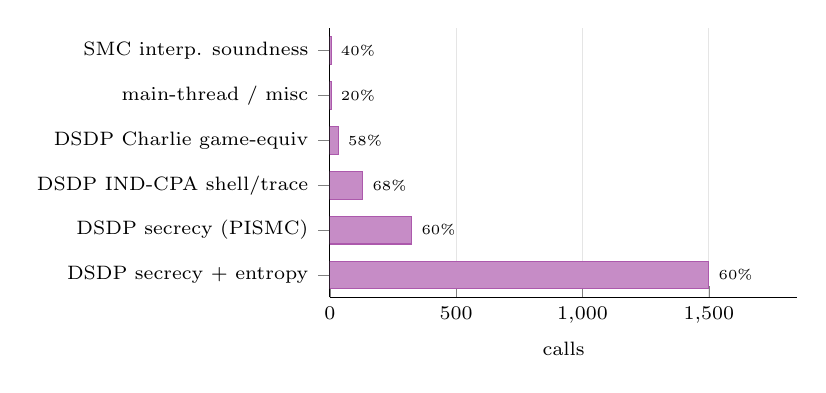
\begin{tikzpicture}
\begin{axis}[xbar, bar width=10pt, width=0.62\linewidth, height=5.0cm, xmin=0, xmax=1850,
  axis x line*=bottom, axis y line*=left, xmajorgrids, grid style={gray!20},
  xlabel={\scriptsize calls}, ytick=data, yticklabels/.expanded={\SessLabels},
  y tick label style={font=\scriptsize}, x tick label style={font=\scriptsize}]
\addplot+[fill=violet!45,draw=violet!65] coordinates {\SessBarCoords};
\SessAnno
\end{axis}
\end{tikzpicture}
\captionof{figure}{rocq-mcp calls per session, labelled by topic; the percentage on
each bar is that session's success rate. The session key below maps each label to
its original (auto-generated) session slug.}\label{fig:sess}
\end{figure}

\noindent\textbf{Session key} (chart label, original slug, volume):
{\small
\begin{itemize}[leftmargin=1.4em,itemsep=1pt,topsep=2pt]
\SessLegend
\end{itemize}}

\section{Intended versus observed behaviour}
\begin{itemize}[leftmargin=1.4em,itemsep=2pt]
\item \textbf{Import caching / sub-second \rcheck{}} (documented): \emph{confirmed},
median \Checkmed\,s.
\item \textbf{\texttt{last\_valid\_state} recovery} (documented): \emph{confirmed},
it is the most common post-failure action (\(416\) times).
\item \textbf{\texttt{force\_restart} ``rarely needed''} (documented): \emph{not
borne out} here. It appears \Forcerestart{} times, frequently after timeouts that
auto-restarted the PET worker.
\item \textbf{\rverify{} rejects custom axioms} (documented safety net):
\emph{never exercised} (0 calls).
\item \textbf{\rstep{} non-destructive, max 20} (documented): consistent with the
observed spray-and-keep pattern.
\end{itemize}

\section{Cross-reference with prior lessons}
The corpus corroborates several already-recorded notes, and surfaces a few new
points. \emph{Confirmed:} the coq-lsp \(\ge0.2.4\) ``No node at point'' bug (the
single biggest failure source, and dated entirely before the 2026-06-02 patch);
PET timeouts on large files (the \rstart{} 30\,s cliff); and the verification
ladder (\rcheck{} an order of magnitude cheaper than compiling). \emph{Not
observable here:} the rocqworker out-of-memory and ``kill does not propagate''
lessons leave no trace in tool results (they are infrastructure events; with
\Nunmatched{} unmatched calls there is no crash signature in this window).
\emph{Novel:} (i) \rquery{} and \rassum{} were not merely flaky but \emph{totally}
down for the window; (ii) the recorded guidance to ``always Search before writing
tactics'' was effectively un-followable through MCP while \rquery{} was broken, a
genuine process gap; (iii) \rverify{}/\rnot{} have never entered the workflow.

\section{Recommendations}
\textbf{Tool-side.}
\begin{enumerate}[leftmargin=1.6em,itemsep=1pt]
\item Treat the ``No node at point'' patch (2026-06-02) as load-bearing: pin the
coq-lsp/pet version and add a one-line smoke test (a \rquery{} ``Check nat.'') so a
future upgrade cannot silently re-break the read-only tools.
\item Raise or stage the 30\,s start timeout for large files, or split files
above \(\sim1000\) lines, to remove the \rstart{} cliff.
\end{enumerate}
\textbf{Usage-side.}
\begin{enumerate}[leftmargin=1.6em,itemsep=1pt]
\item Adopt \rverify{} at proof-close: it is the cheapest guard against custom
axioms and statement drift, and it is currently unused.
\item Use \rnot{} when a notation-ambiguity error appears, instead of guessing.
\item Keep leaning on \rcheck{} (fast, reliable) and \rstep{} for exploration; the
data shows this loop works.
\end{enumerate}
\textbf{Process-side.} Re-run \texttt{parse.py} after each burst of work; watch for
\texttt{force\_restart} spikes and \(\ge3\)-failure runs as early signals of a
stuck session.

\appendix
\section{Per-tool table}
\begin{table}[h]\centering\small
\begin{tabular}{lrrrrrrr}
\toprule
tool & calls & succ & fail & unk & unmatch & succ\% & med\,(s)\\
\midrule
\ToolTableRows
\bottomrule
\end{tabular}
\captionof{table}{Per-tool counts and median latency.}
\end{table}

\section{By agent type}
\begin{table}[h]\centering\small
\begin{tabular}{lrr}
\toprule
agent type & calls & succ\%\\
\midrule
\AttrTableRows
\bottomrule
\end{tabular}
\captionof{table}{Calls and success rate by attributed agent type.}
\end{table}

\noindent\emph{Reproducibility.} All figures derive from \texttt{parse.py}
(read only) over the project's transcript directory under
\texttt{\textasciitilde/.claude/projects/}. It writes \texttt{metrics.tex}
(consumed here), \texttt{metrics.json}, and \texttt{samples.txt}, and self-checks
its counts against grep priors and a \(>90\%\) subagent-share gate before emitting
anything.

\end{document}
